\documentclass[14pt]{extbook}
\usepackage{multicol, enumerate, enumitem, hyperref, color, soul, setspace, parskip, fancyhdr} %General Packages
\usepackage{amssymb, amsthm, amsmath, latexsym, units, mathtools} %Math Packages
\everymath{\displaystyle} %All math in Display Style
% Packages with additional options
\usepackage[headsep=0.5cm,headheight=12pt, left=1 in,right= 1 in,top= 1 in,bottom= 1 in]{geometry}
\usepackage[usenames,dvipsnames]{xcolor}
\usepackage{dashrule}  % Package to use the command below to create lines between items
\newcommand{\litem}[1]{\item#1\hspace*{-1cm}\rule{\textwidth}{0.4pt}}
\pagestyle{fancy}
\lhead{Makeup Progress Quiz 2}
\chead{}
\rhead{Version C}
\lfoot{2790-1423}
\cfoot{}
\rfoot{Summer C 2021}
\begin{document}

\begin{enumerate}
\litem{
Which of the following equations \textit{could} be of the graph presented below?
\begin{center}
    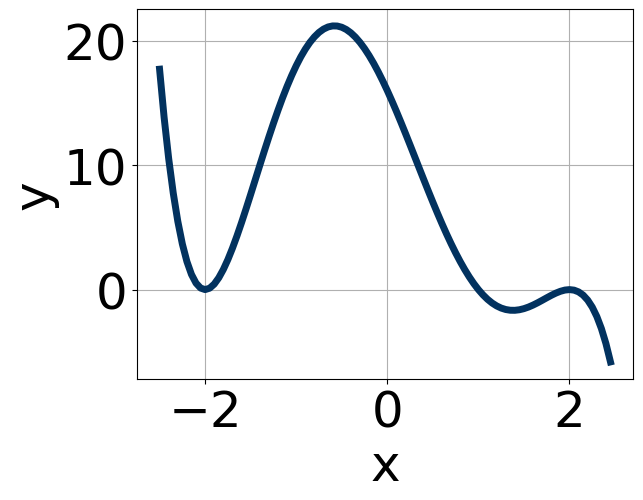
\includegraphics[width=0.5\textwidth]{../Figures/polyGraphToFunctionC.png}
\end{center}
\begin{enumerate}[label=\Alph*.]
\item \( -13(x - 2)^{10} (x + 2)^{5} (x - 1)^{10} \)
\item \( -14(x - 2)^{10} (x + 2)^{9} (x - 1)^{11} \)
\item \( 18(x - 2)^{10} (x + 2)^{4} (x - 1)^{10} \)
\item \( -6(x - 2)^{10} (x + 2)^{4} (x - 1)^{7} \)
\item \( 16(x - 2)^{8} (x + 2)^{8} (x - 1)^{5} \)

\end{enumerate} }
\litem{
Construct the lowest-degree polynomial given the zeros below. Then, choose the intervals that contain the coefficients of the polynomial in the form $ax^3+bx^2+cx+d$.\[ \frac{-3}{5}, \frac{7}{4}, \text{ and } \frac{1}{3} \]\begin{enumerate}[label=\Alph*.]
\item \( a \in [53, 63], b \in [-91, -78], c \in [-46, -37], \text{ and } d \in [-21, -18] \)
\item \( a \in [53, 63], b \in [-91, -78], c \in [-46, -37], \text{ and } d \in [20, 23] \)
\item \( a \in [53, 63], b \in [83, 95], c \in [-46, -37], \text{ and } d \in [-21, -18] \)
\item \( a \in [53, 63], b \in [49, 51], c \in [-88, -79], \text{ and } d \in [20, 23] \)
\item \( a \in [53, 63], b \in [-165, -159], c \in [107, 112], \text{ and } d \in [-21, -18] \)

\end{enumerate} }
\litem{
Describe the zero behavior of the zero $x = 8$ of the polynomial below.\[ f(x) = 3(x + 8)^{8}(x - 8)^{11}(x - 7)^{9}(x + 7)^{13} \]\begin{enumerate}[label=\Alph*.]
\begin{multicols}{2}\item 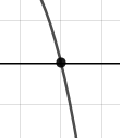
\includegraphics[width = 0.3\textwidth]{../Figures/polyZeroBehaviorCopyAC.png}\item 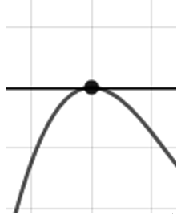
\includegraphics[width = 0.3\textwidth]{../Figures/polyZeroBehaviorCopyBC.png}\item 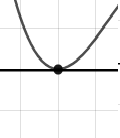
\includegraphics[width = 0.3\textwidth]{../Figures/polyZeroBehaviorCopyCC.png}\item 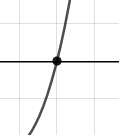
\includegraphics[width = 0.3\textwidth]{../Figures/polyZeroBehaviorCopyDC.png}\end{multicols}\item None of the above.
\end{enumerate} }
\litem{
Describe the end behavior of the polynomial below.\[ f(x) = -4(x + 6)^{4}(x - 6)^{5}(x + 2)^{5}(x - 2)^{5} \]\begin{enumerate}[label=\Alph*.]
\begin{multicols}{2}\item 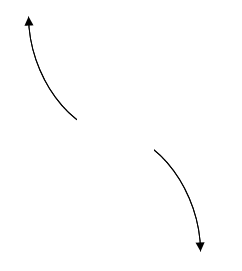
\includegraphics[width = 0.3\textwidth]{../Figures/polyEndBehaviorCopyAC.png}\item 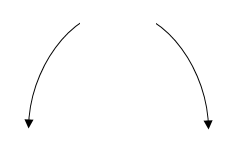
\includegraphics[width = 0.3\textwidth]{../Figures/polyEndBehaviorCopyBC.png}\item 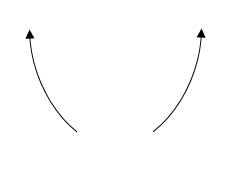
\includegraphics[width = 0.3\textwidth]{../Figures/polyEndBehaviorCopyCC.png}\item 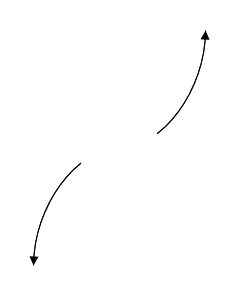
\includegraphics[width = 0.3\textwidth]{../Figures/polyEndBehaviorCopyDC.png}\end{multicols}\item None of the above.
\end{enumerate} }
\litem{
Describe the end behavior of the polynomial below.\[ f(x) = 4(x + 2)^{5}(x - 2)^{8}(x + 9)^{3}(x - 9)^{3} \]\begin{enumerate}[label=\Alph*.]
\begin{multicols}{2}\item 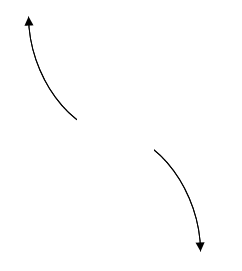
\includegraphics[width = 0.3\textwidth]{../Figures/polyEndBehaviorAC.png}\item 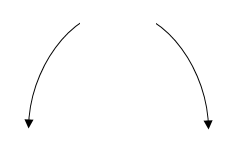
\includegraphics[width = 0.3\textwidth]{../Figures/polyEndBehaviorBC.png}\item 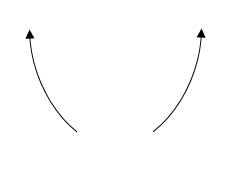
\includegraphics[width = 0.3\textwidth]{../Figures/polyEndBehaviorCC.png}\item 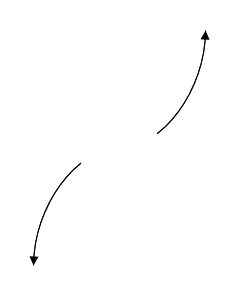
\includegraphics[width = 0.3\textwidth]{../Figures/polyEndBehaviorDC.png}\end{multicols}\item None of the above.
\end{enumerate} }
\litem{
Construct the lowest-degree polynomial given the zeros below. Then, choose the intervals that contain the coefficients of the polynomial in the form $x^3+bx^2+cx+d$.\[ -5 + 5 i \text{ and } -1 \]\begin{enumerate}[label=\Alph*.]
\item \( b \in [-16, -10], c \in [59, 67], \text{ and } d \in [-58, -48] \)
\item \( b \in [4, 19], c \in [59, 67], \text{ and } d \in [46, 58] \)
\item \( b \in [-8, 6], c \in [-1, 13], \text{ and } d \in [3, 6] \)
\item \( b \in [-8, 6], c \in [-6, 3], \text{ and } d \in [-7, 3] \)
\item \( \text{None of the above.} \)

\end{enumerate} }
\litem{
Construct the lowest-degree polynomial given the zeros below. Then, choose the intervals that contain the coefficients of the polynomial in the form $ax^3+bx^2+cx+d$.\[ \frac{-2}{5}, \frac{-3}{2}, \text{ and } \frac{1}{5} \]\begin{enumerate}[label=\Alph*.]
\item \( a \in [48, 62], b \in [44, 50], c \in [-44, -38], \text{ and } d \in [1, 10] \)
\item \( a \in [48, 62], b \in [-106, -98], c \in [42, 50], \text{ and } d \in [-8, 2] \)
\item \( a \in [48, 62], b \in [79, 88], c \in [7, 18], \text{ and } d \in [-8, 2] \)
\item \( a \in [48, 62], b \in [79, 88], c \in [7, 18], \text{ and } d \in [1, 10] \)
\item \( a \in [48, 62], b \in [-85, -84], c \in [7, 18], \text{ and } d \in [1, 10] \)

\end{enumerate} }
\litem{
Which of the following equations \textit{could} be of the graph presented below?
\begin{center}
    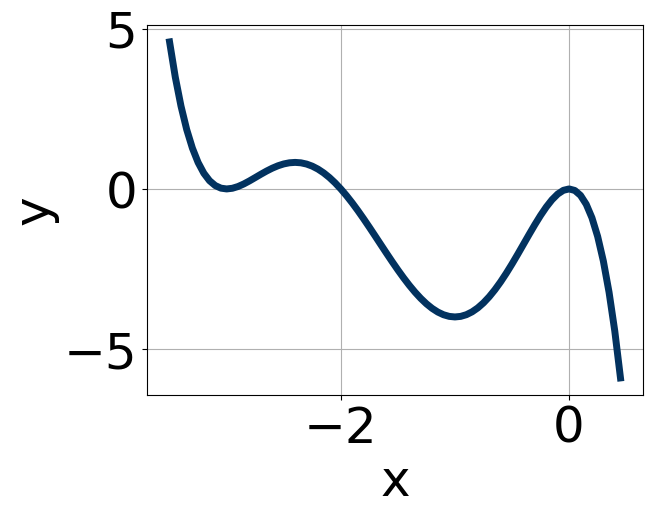
\includegraphics[width=0.5\textwidth]{../Figures/polyGraphToFunctionCopyC.png}
\end{center}
\begin{enumerate}[label=\Alph*.]
\item \( 14x^{10} (x + 3)^{10} (x + 2)^{5} \)
\item \( 18x^{10} (x + 3)^{4} (x + 2)^{4} \)
\item \( -11x^{9} (x + 3)^{6} (x + 2)^{5} \)
\item \( -13x^{8} (x + 3)^{10} (x + 2)^{5} \)
\item \( -8x^{11} (x + 3)^{10} (x + 2)^{10} \)

\end{enumerate} }
\litem{
Construct the lowest-degree polynomial given the zeros below. Then, choose the intervals that contain the coefficients of the polynomial in the form $x^3+bx^2+cx+d$.\[ 4 - 3 i \text{ and } 3 \]\begin{enumerate}[label=\Alph*.]
\item \( b \in [9, 12], c \in [40, 52], \text{ and } d \in [74, 86] \)
\item \( b \in [-14, -5], c \in [40, 52], \text{ and } d \in [-77, -72] \)
\item \( b \in [0, 3], c \in [0, 5], \text{ and } d \in [-9, -8] \)
\item \( b \in [0, 3], c \in [-10, -6], \text{ and } d \in [7, 16] \)
\item \( \text{None of the above.} \)

\end{enumerate} }
\litem{
Describe the zero behavior of the zero $x = 3$ of the polynomial below.\[ f(x) = 3(x - 3)^{5}(x + 3)^{10}(x + 8)^{5}(x - 8)^{6} \]\begin{enumerate}[label=\Alph*.]
\begin{multicols}{2}\item 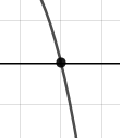
\includegraphics[width = 0.3\textwidth]{../Figures/polyZeroBehaviorAC.png}\item 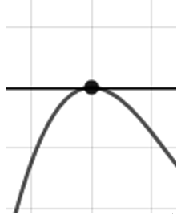
\includegraphics[width = 0.3\textwidth]{../Figures/polyZeroBehaviorBC.png}\item 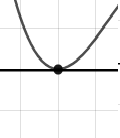
\includegraphics[width = 0.3\textwidth]{../Figures/polyZeroBehaviorCC.png}\item 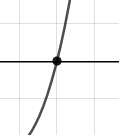
\includegraphics[width = 0.3\textwidth]{../Figures/polyZeroBehaviorDC.png}\end{multicols}\item None of the above.
\end{enumerate} }
\end{enumerate}

\end{document}